\documentclass[a4paper]{article}
\usepackage[cm]{fullpage}
\usepackage{graphicx}
\usepackage{bm}
\usepackage{multicol}

\begin{document}
\begin{center}
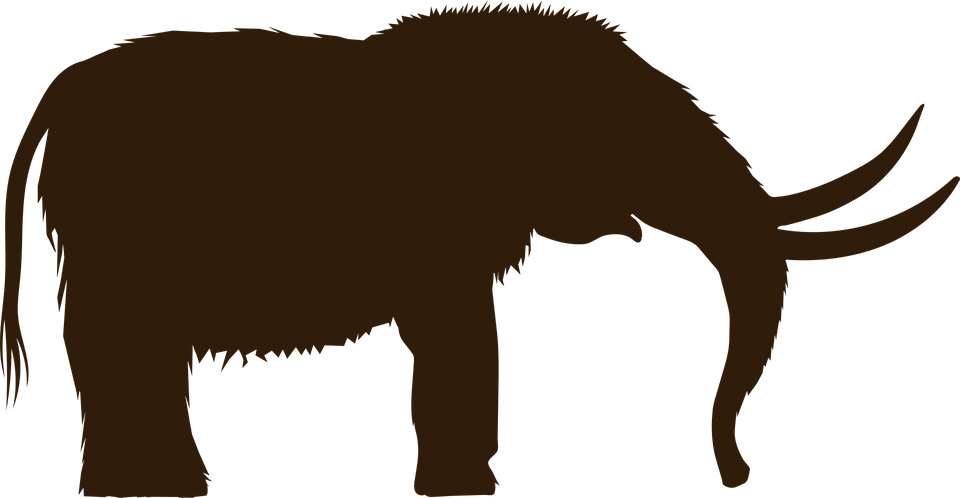
\includegraphics[width=10cm]{mammoth}\\
\vspace{4cm}
{\Large MAMMOTH}\\
C. Thieulot\\
Utrecht Universiteit
\end{center}

%===========================================================
\newpage
\section{Install \& run procedure}

To obtain the code, type the following in the terminal:
\begin{verbatim}
git clone https://github.com/cedrict/mammoth.git
\end{verbatim}
This creates a {\it mammoth} folder. Do
\begin{verbatim}
cd mammoth
\end{verbatim}
To compile the code, simply open a terminal and make sure you have the gfortran compiler installed.
Then simply do
\begin{verbatim}
make
\end{verbatim}
Unless there is an error, this should generate the executable file {\it mammoth}.
To run the executable, simply do
\begin{verbatim}
./mammoth
\end{verbatim}
If you wish to redirect the standard output to a file (e.g. {\it opla}), then:
\begin{verbatim}
./mammoth > opla
\end{verbatim}
If you wish to clean all the data files after a run, use the {\it cleandata} script as follows:
\begin{verbatim}
./cleandata
\end{verbatim}
To clean the code off data and other compilations files:
\begin{verbatim}
make clean
\end{verbatim}
When the code runs it produces ascii data ({\it *.dat} files) and 
paraview files ({\it *.vtu} files) in the {\sl OUT} folder. 
The former can be visualised with gnuplot, while the latter should be opened
with paraview (or VisIt or MayaVi).



%===========================================================
\newpage
\section{Physical equations}

The code solves the heat transport equation in the absence of advective processes:
\[
\rho c_P \frac{\partial T}{\partial t} = {\bm \nabla} \cdot k{\bm \nabla}T + H
\]
where $\rho$ is the mass density (kg/m$^3$), $c_P$ is the heat capacity (), $k$ is the heat conductivity,
and $H$ is a heat production term. $T(x,y,z,t)$ is the temperature field.
The domain is designated by $\Omega$ and its boundary by $\Gamma$.
This PDE must be supplied with boundary conditions: at a given point of the boundary $\Gamma$
either a temperature can be prescribed or a heat flux. 

%===========================================================
\section{Discretisation}

The heat transport equation is solved by means of the Finite Element Method, following 
the methodology presented in \cite{thie11}. The FE equation corresponding to this PDE
is 
\[
{\bm M}\cdot \frac{\partial {\bm T}}{\partial t} + {\bm K}_d \cdot {\bm T} = {\bm F}
\]
where 
\[
{\bm M}=\int_\Omega {\bm N}^T \rho c_P {\bm N} dV
\]
\[
{\bm K}_d=\int_\Omega {\bm B}^T k {\bm B} dV
\]
\[
{\bm F} = \int_\Omega {\bm N}^T H dV
\]
where ${\bm T}$ is the vector of nodal temperatures.

The domain $\Omega$ of size $L_x\times L_y\times L_z$
is divided into $nel=nelx\times nely\times nelz$ elements as shown hereunder. 
The computational grid therefore counts $np=(nelx+1)(nely+1)(nelz+1)$ nodes and as many degrees of freedom.
A Cartesian coordinate system is used with its origin at the bottom corner of the domain.

\begin{center}
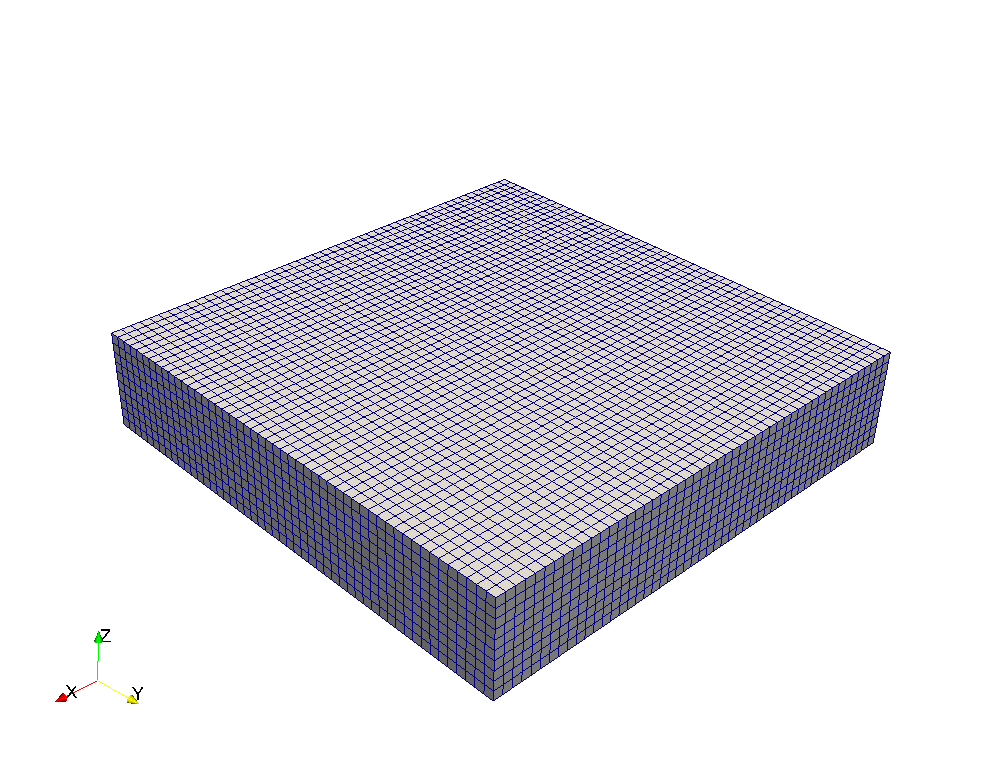
\includegraphics[width=15cm]{grid}
\end{center}

%===========================================================
\section{Setting up an experiment}

\subsection{Initial temperature field}


\subsection{Magma chambers}

The code can model as many magma chambers as needed. This number is controlled by the 
{\tt nchamber} parameter.
Each chamber is parametrised by:
\begin{itemize}
\item its {\tt shape}: 1 is a spheroid, 2 is a cuboid and 3 is a cylinder;  
\item its center coordinates {\tt xc}, {\tt yc}, {\tt zc};
\item its spatial extent in the $x$, $y$, $z$ directions: {\tt a}, {\tt b} and {\tt c};
\item its initial temperature {\tt T}.
\end{itemize}

\paragraph{Example} The following figure is obtained by setting three magma chambers as follows:

\begin{multicols}{2}


\begin{verbatim}
mc(1)%shape=1
mc(1)%xc=0.5*Lx
mc(1)%yc=0.5*Ly
mc(1)%zc=0.5*Lz
mc(1)%a=4d3
mc(1)%b=5d3
mc(1)%c=6d3
mc(1)%T=500

mc(2)%shape=2
mc(2)%xc=0.25*Lx
mc(2)%yc=0.2*Ly
mc(2)%zc=0.4*Lz
mc(2)%a=10d3
mc(2)%b=5d3
mc(2)%c=4d3
mc(2)%T=500

mc(3)%shape=3
mc(3)%xc=0.7*Lx
mc(3)%yc=0.33*Ly
mc(3)%zc=0.6*Lz
mc(3)%a=8d3
mc(3)%b=8d3
mc(3)%c=3d3
mc(3)%T=500
\end{verbatim}

\begin{center}
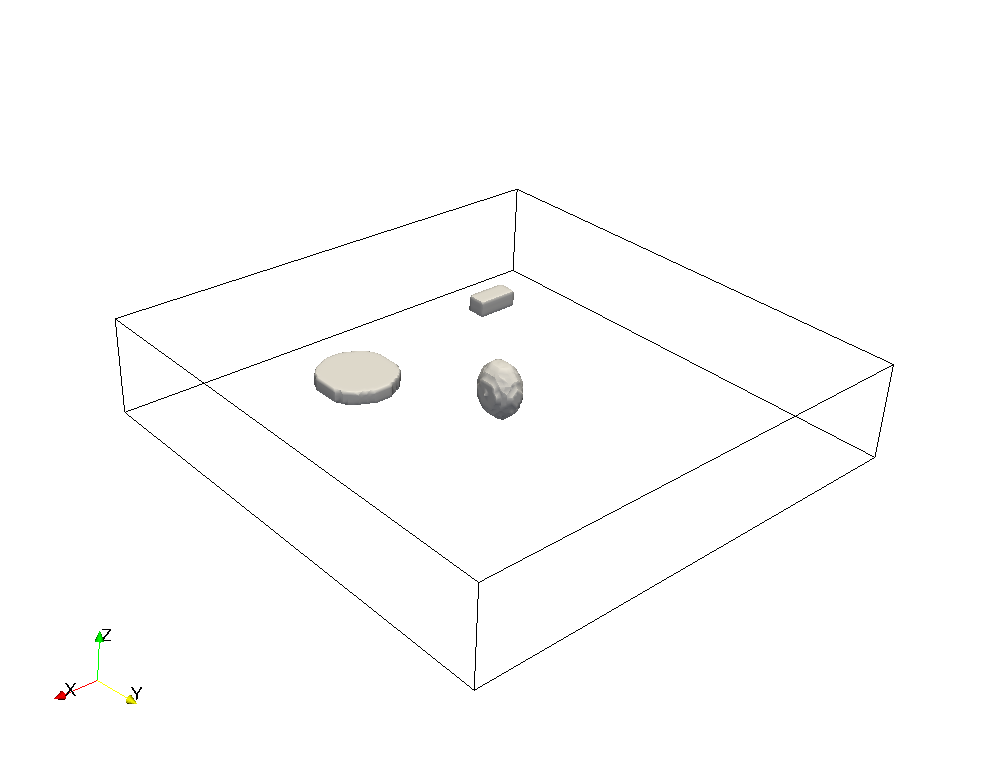
\includegraphics[width=8cm]{threechambers}
\end{center}
\end{multicols}

\subsection{Boundary conditions}





%===========================================================
\appendix
\newpage
\section{Steady state solutions}

%--------------------------
\subsection{One layer}

At steady state: $\partial T/\partial t=0$ so that one has to solve 
\[
\Delta T = -\frac{H}{k}
\]
Assuming the domain to be infinite in the $x$ and $y$ direction this equation becomes:
\[
\frac{d^2T}{dz^2} = -\frac{H}{k}
\]
The generic solution to this ODE is given by:
\begin{equation}
T(z)=-\frac{H}{2k} z^2 + Az +B
\label{eq:gs1}
\end{equation}
where $A$ and $B$ are integration constants to be determined by means of the specified boundary conditions.

At the surface a constant temperature is maintained, i.e. $T(z=L)=T_s$, so that 
\[
T(L)=-\frac{H}{2k} L^2 + AL +B = T_s
\]
which allows us to express $B$ as a function of the rest and insert back into Eq. (\ref{eq:gs1}):
\[
T(z)=-\frac{H}{2k} (z^2-L^2) + A(z-L) + T_s
\]

\paragraph{Temperature prescribed at the bottom}

In this case $T(z=0)=T_b$ so that
\[
T(z)=-\frac{H}{2k} L^2 + AL + T_s=T_b
\]
which yields 
\[
A=\frac{T_b-T_s}{L} + \frac{HL}{2k}
\]
 

\paragraph{Heat flux prescribed at the bottom}

In this case $kdT/dz(z=0)=\phi_b$ which yields $kA=\phi_b$ so that
\[
T(z)=-\frac{H}{2k} (z^2-L^2) + \frac{\phi_b}{k}(z-L) + T_s
\]


%--------------------------
\subsection{Two layers}

In each layer $i$ the solution is given by:
\begin{equation}
T(z)=-\frac{H_i}{2k_i} z^2 + A_iz +B_i \label{eq:gs2}
\end{equation}
Aside from the two previous boundary conditions we need to enforce that the temperature and the heat flux 
are continuous fields, .i.e. $T(z=l^-)=T(z=l^+)$ and $\phi(z=l^-)=\phi(z=l^+)$.

%%%%%%%%%%%%%%%%%%%%%%%%%%%%%%%%%%%%%%%%%%%%%%%%%%%%%55
\newpage
\section{todo}




\end{document}
